\section{Revised Block Diagram}

Figure~\ref{fig:blockDiagram} shows a revised system block diagram.  It contains the model numbers of the known components, the type of connection required to the microcontroller unit and the amount of lines needed for each connection.  Several components such as the power management circuit, battery meter and charger are still to be chosen as several methods of battery charging are being considered.

%TODO Fix amount of lines in block diagram
\begin{figure}[H]
	\centering
	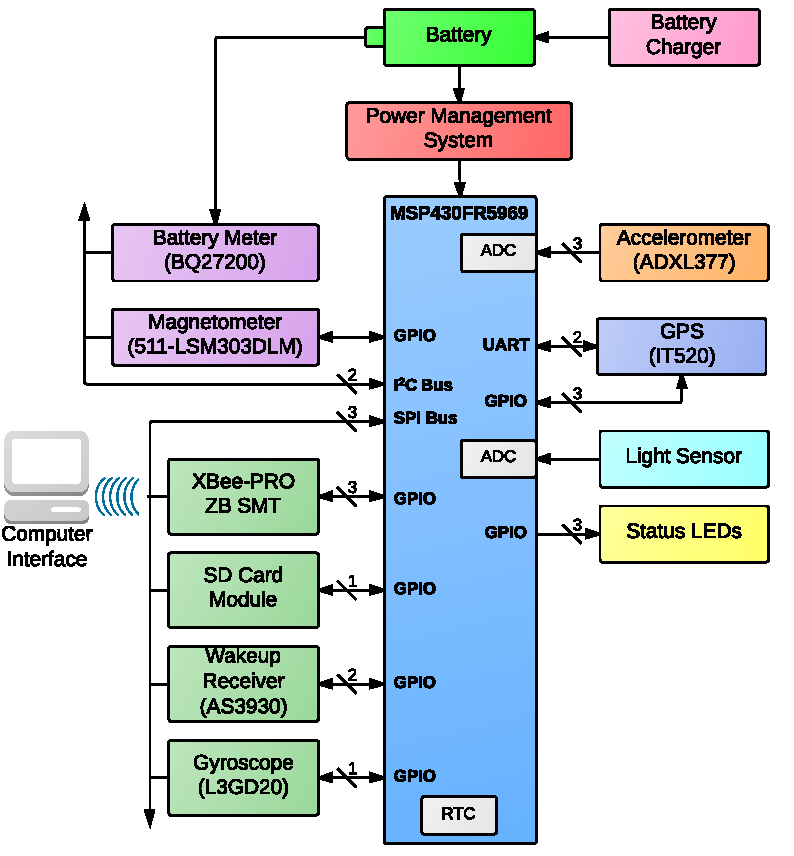
\includegraphics[width=\textwidth]{img/blockDiagramV2_2}
	\caption{Revised Block Diagram \label{fig:blockDiagram}}
\end{figure}

\subsection{Battery Charging Methods}
Two different methods are being considered for charging the sphere's battery.
\subsubsection{USB Charger}
\subsubsection{Wireless Charger}
Wireless charging involves charging the sphere's battery without being physically connected to an outlet or to another device. The reason this method is being considered is because if the device is wirelessly charged then the device wouldn't need an external port that would be use to charge the device without opening the sphere and if no external port is used then it wouldn't also be needed for the user to physically open the sphere and disconnect the battery to charge it somewhere else. Exploring the idea we discovered the Qi (pronounced \'chee\') standard which dictates a wireless charging and communication interface. Qi standards mention that the energy transfer must occur to a distance up to 40 millimeters and that the primary inductive coil must be flat in a spiral formation \cite{QiStandard}. With such constrains the Qi standard is discarded and because furthermore the standard is intended to be used for multiple devices with different power requirements, Qi has a communication protocol that complicate the devices and obligates us to integrate further IC that can potentially use space. Discarding Qi lead us to consider implementing a custom wireless charger, the idea is to basically transfer energy from a 120V AC outlet trough a transformer into the spheres. The transformer will actually be two separated coils which by inductance can transfer energy at a long distance. An AC current will be created inside the sphere's coil which will then have to be rectified into a DC current that can charge the device's battery. Various factors are to be considered when implementing such charger, energy transferring by inductance is not very efficient, the coils require specific geometry and number of turns, moreover the frequency in which the current changes in the primary coil must be specific, such ideal resonance frequency is needed to archive maximum energy transfer. Research and experiments are being performed to converge into an implementation, it is possible to supply the primary coil with a controlled oscillating DC current that would still cause the necessary change in flux to create an inductive charge. Ideally the user will have a charge station that will be connected to a power outlet and can hold a few spheres, each sphere being hold by such charging station is being charged wirelessly without the need of connecting it or opening it. 
